\chapter{\IfLanguageName{dutch}{Continuous Integration, Continuous Delivery \& Continuous Deployment}{Continuous Integration, Continuous Delivery \& Continuous Deployment}}
\label{ch:ci-cd-cd}
    \section{Algemeen}
    \label{sec:algemeen}
    Bedrijven zijn constant op zoek naar betere en snellere resultaten. In het software development circuit is het vandaag soms nog lang wachten voor een wijziging effectief doorgevoerd wordt. Men levert nog vaak software op aan het einde van de sprint, wat soms voor problemen zorgt als men veel code tegelijk aflevert. Met een nieuwe software development methode - Continuous Integration en Continuous Delivery genaamd - wil men deze problemen zoveel mogelijk vermijden. Er wordt vaak gesproken van een CI/CD pipeline als het gaat over Continuous Integration en Continuous Delivery, maar er is nog een derde speler dat men kan invoeren: Continuous Deployment. Samen vormen zij de 3 musketiers om software projecten een grotere slaagkans te geven.
    Om een duidelijker beeld te scheppen van een CI/CD pipeline zal dit hoofdstuk eerst uitleg verschaffen over DevOps, omdat dit de allesomvattende term is waar de 3 musketiers deel van uitmaken. Er wordt ook dieper ingegaan op Continuous Integration, Continuous Delivery, Continuous Deployment en tot slot komt Automated Testing aan bod.
        \paragraph{DevOps}
        DevOps is een samentrekking van development en operations en is een welbekend begrip binnen de informatica wereld. Het heeft als doel om de 'state of mind' binnen een bedrijf te veranderen zodat alle lagen/departementen vlotter samenwerken. Het is een praktische 'gids' dat bedrijven kunnen gebruiken om de communicatie tussen developers en systeembeheerders beter te maken. Deze twee verschillende lagen in een bedrijf willen namelijk hetzelfde: zo snel mogelijk kwaliteitsvolle software opleveren. DevOps is gebaseerd op Agile development, maar gaat verder dan dat. Het gaat dieper in op automatisatie, integratie, samenwerking en communicatie. 
        Continuous Integration, Delivery en Deployment zijn kenmerkend voor DevOps, omdat het mee inzet op snellere oplevering van kwaliteitsvolle software. ~\autocite{Riti2018}
    
        \paragraph{Continuous Integration}
        Dit is een eerste stap in de pipeline waarbij de geschreven code wordt gecommit naar een 'repository management server'. Hierdoor wordt de 'source code' automatisch opnieuw opgebouwd en slaagt voor de testen die automatisch zijn opgestart. De focus bij deze stap ligt bij de teamleden ~\autocite{Fowler2006}, van hen wordt verwacht dat ze - op regelmatige basis - hun code pushen (integreren met de master applicatie). Een goede samenwerking tussen de verschillende leden van het development team is broodnodig om tot het gewenste eindresultaat te komen.
        Het doel van een Continuous Integration is om de integratie feilloos te laten verlopen wanneer men software ontwikkelt en geen functionaliteiten verliezen na een merge ~\autocite{Riti2018}.
        
        Bovenstaande uitleg is makkelijker te begrijpen aan de hand van een voorbeeld. Op Figuur \ref{img-ci-example} is een grafische voorstelling van dit voorbeeld terug te vinden.
        De developer maakt een wijziging en commit de code naar de repository die te vinden is op het source-control systeem. De Continuous Integration server krijgt het bericht dat er code is toegevoegd, haalt de laatst toegevoegde code op en laat de testen runnen. Wanneer alle testen slagen zal de CI server de code compilen en feedback bezorgen aan de developer. In dit voorbeeld is er gebruik gemaakt van een externe mail server om die feedback te verzenden.
        Deze stappen gebeuren elke keer er code naar de repository gestuurd wordt.
        Bovenstaand voorbeeld is een best-practice hoe het zou moeten gebeuren. Er zijn echter enkele zaken die wat extra uitleg kunnen gebruiken.
        De frequentie en hoeveelheid code zijn belangrijke zaken waar de developer rekening mee moet houden bij een CI pipeline. Volgens \textcite{Fowler2006} is het de plicht van een developer om minstens 1 maal per dag een commit te doen. Hij moet telkens een commit uitvoeren wanneer hij een kleine opdracht afgerond heeft. Zo blijft de hoeveelheid code klein en is het makkelijk om te zoeken wanneer er zich een probleem voordoet.
        Eens de wijziging gecommit is naar de version control repository moet de CI pipeline zijn werk doen. Een belangrijke stap is het bezorgen van de feedback. Dit moet namelijk het resultaat van de build en de feedback waar het probleem zich kan bevinden terug geven, door bijvoorbeeld aan te geven welke test niet slaagt bij het uitvoeren van de automated testing. De key factor hier is de tijd. Als de developer pas daags nadien feedback krijgt over de fout die hij gepusht heeft, wordt het al moeilijker om de fout te vinden en ze op te lossen. 
        \begin{figure}	
            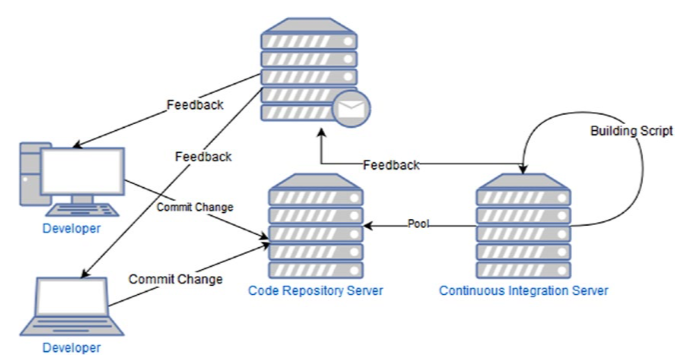
\includegraphics[scale=0.65]{ci-example}
            \caption{Voorbeeld van een Continuous Integration set-up ~\autocite{Riti2018}} \label{img-ci-example}
        \end{figure}
    
        \paragraph{Continuous Delivery}
        Eens het team met succes de Continuous Integration toepast kan men overschakelen naar de volgende stap: Continuous Delivery.
        Het is een manier dat ervoor zorgt dat de code die van de Continuous Integration stap komt, gebuild en voorbereid wordt voor een release.
        Er is echter wel nog een menselijke hand nodig om de build van deze stap te deployen en voor de buitenwereld beschikbaar te stellen ~\autocite{Fowler2013}.
        \newline{}In Figuur \ref{img-cd-chain} wordt de opbouw van een Continuous Delivery chain weergegeven, het is een grafische weergave van de stappen die een Continuous Delivery pipeline moet hebben. Dit is gebaseerd op de Continuous Integration chain, maar hier zijn extra stappen toegevoegd.
        De eerste stap is het developen van de code die men wenst op te leveren. Net zoals bij Continuous Integration commit de developer de code naar de version control repository. De build scheduler haalt de laatst toegevoegde code op en test deze code. Enkel bij het slagen van alle testen wordt de code gebuild door de build scheduler. Deze maakt ook de build klaar voor release en vereist enkel nog menselijke goedkeuring om deze release te lanceren.
        \newline{}In dit proces is feedback ook uiterst belangrijk. Wanneer developers foute code pushen, moet de persoon die de foute code geschreven heeft zo snel mogelijk verwittigd worden. Op deze manier kan het euvel snel opgelost worden.
        Mail kan een vorm zijn van feedback, maar er bestaan nog andere leuke vormen naast mailing. Het bedrijf Dynatrace heeft bijvoorbeeld een licht ontworpen dat je in de kamer van het team kan hangen. Dit Internet of Things (IoT) gadget, DevOps UFO genaamd, is via WiFi verbonden aan de pipeline omgeving. Het geeft feedback over de staat van de CI/CD pipeline en is een vorm van monitoring. Het geeft de developers en iedereen in de kamer onmiddelijke feedback wanneer er een commit gebeurd. Als de commit door de pipeline geraakt zal de UFO groen kleuren, wanneer de build faalt kleurt de UFO rood en weet iedereen dat er een fout is. Zo weet de persoon die de foute code gepusht heeft dat er iets fout is en kan hij hier nog sneller op inspelen. 
        \begin{figure}	
            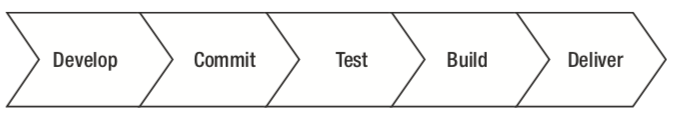
\includegraphics[scale=0.65]{cd-chain}
            \caption{Continuous Delivery chain ~\autocite{Riti2018}} \label{img-cd-chain}
        \end{figure}
        
        \paragraph{Continuous Deployment}
        De gelijkenis met Continuous Deployment is treffend, maar er is wel degelijk een verschil.
        Hier gaat men automatisch de veranderde code naar productie brengen. De veranderingen gaan door de volledige pipeline en eens ze slagen voor alle testen wordt - zonder menselijke interactie - de code naar productie gebracht ~\autocite{Claps2015}.
        Dit wordt soms ook wel de 'train to production' genoemd, omdat elke code dat gepusht wordt naar de source-control automatisch tot bij de klant geraakt.
        
        \paragraph{Automated Testing}
        Zoals hierboven reeds aangegeven is er geen Continuous Integration pipeline zonder automated testing. Het grootste doel van deze fase is - zoals de naam het zegt - testen van de code. Als de CI/CD pipeline voorzien wordt van voldoende en goede testen, wordt er een veiligheidsgevoel gecreëerd. Op deze manier voldoet de software aan bepaalde criteria, die in de testen verwerkt worden. Het is dus een heel belangrijk onderdeel van de pipeline waar veel aandacht aan besteed moet worden. 
        Om te voldoen aan de criteria van CI/CD moeten de testen automatisch gerund worden. Dit was tot voor kort echter vaak niet het geval. Er waren testers aangesteld om telkens opnieuw software te testen, door op de verschillende knoppen te drukken in de user interface (UI). Heel vaak slopen er fouten in omdat dit heel repetitief en saai werk was. Daar komt de automatisatie van pas ~\autocite{Vocke2018}.
        
        Mike Cohn kwam met het idee om testen op te delen in drie grote categorieën: Unit Tests, Service Tests en UI tests zoals u kan zien in Figuur \ref{img-test-pyramid}.
        Vandaag zijn deze categorieën iets te simplistisch voorgesteld, vanwege de toenemende complexiteit van de software. Maar het is wel nog altijd een uitstekende referentie om de opbouw van testen uit te leggen.
        Twee zaken zijn belangrijk om te onthouden: testen moeten uit verschillende lagen van detail bestaan en er moeten minder testen geschreven worden wanneer het team minder gedetailleerd (high-level testing) gaat. Omdat bij high-level testen de requirements goed begrepen zijn door het test team.
        De grootste laag binnen de test omgeving zijn de Unit tests en staat het dichts bij de software code. Deze testen zijn snel om te schrijven en te runnen en kunnen gedetailleerde feedback geven wanneer een test faalt.
        De laag erboven service tests - ook wel Integration tests genoemd - focust vooral op de functionaliteit van de applicatie.
        Deze testen leggen de nadruk op de functionaliteit dat de applicatie moet bevatten. Ze testen de API calls en de integratie van de individuele functies.
        De kleinste laag zijn de UI tests, ook wel end-to-end testen genoemd. Deze testen de user interface door bijvoorbeeld op knoppen te drukken, formulieren in te vullen of te navigeren doorheen de applicatie. Het nadeel van deze testen zijn dat ze fragiel, duur en tijdrovend zijn om te bouwen en traag om te runnen zijn.
        Om de snelheid te garanderen en de hoeveelheid build times klein te houden is het belangrijk de vorm van de piramide te behouden. Het gevaar dreigt om de test omgeving als een ijsjes hoorn te vormen met meer UI tests dan Unit tests ~\autocite{Fowler2012}.
        \begin{figure}	
            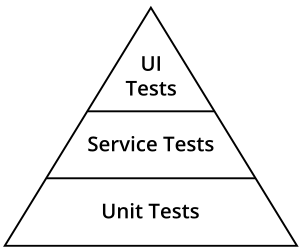
\includegraphics[scale=0.65]{test-pyramid}
            \caption{Test piramide ~\autocite{Vocke2018}} \label{img-test-pyramid}
        \end{figure}